\documentclass[12pt]{article}

\usepackage[active]{srcltx}

\usepackage{amsmath,amsfonts,amssymb,amsthm}
\usepackage{easybmat}
\usepackage{graphicx}
%\usepackage[hypertex]{hyperref}
%\usepackage[pdftex]{hyperref}
\usepackage{fancyhdr}
\usepackage{subfigure}

\usepackage{makeidx}
\makeindex

\theoremstyle{plain}
\newtheorem{theorem}{Theorem}
\newtheorem{property}[theorem]{Property}
\newtheorem{condition}[theorem]{Condition}
\newtheorem{proposition}[theorem]{Proposition}
\newtheorem{axiom}[theorem]{Axiom}
\newtheorem{lemma}[theorem]{Lemma}
\newtheorem{corollary}[theorem]{Corollary}
%%
% % Make numbering specific to the Appendix
% \newtheorem{Atheorem}{Theorem}[chapter]
% \newtheorem{Aproperty}[Atheorem]{Property}
% \newtheorem{Acondition}[Atheorem]{Condition}
% \newtheorem{Aproposition}[Atheorem]{Proposition}
% \newtheorem{Aaxiom}[Atheorem]{Axiom}
% \newtheorem{Alemma}[Atheorem]{Lemma}
% \newtheorem{Acorollary}[theorem]{Corollary}

% Make definitions non italicized
%\theoremstyle{definition}
\newtheorem{definition}[theorem]{Definition}
% Make numbering specific to the Appendix
%\newtheorem{Adefinition}[Atheorem]{Definition}
\newenvironment{defi}{\vskip0.2cm\addtocounter{theorem}{1}\par\noindent\bf Definition~\arabic{section}.\arabic{subsection}.\arabic{theorem}\rm.}{\hfill{$\circ$}\par\vskip0.25cm}


%% Example environment and counter.
\newcounter{cmpt_exercise}
\newenvironment{exercise}{\addtocounter{cmpt_exercise}{1}\vskip0.2cm\par\noindent\begin{small}\bf Exercise~\arabic{cmpt_exercise}\,\,\rm --}{\hfill{$\circ$}\end{small}\par\vskip0.25cm}
\newenvironment{problem}{\addtocounter{cmpt_exercise}{1}\vskip0.2cm\par\noindent{\Large\bf Problem~\arabic{cmpt_exercise}\,\,\rm --}}{\par\vskip0.25cm}


\newenvironment{example}{\vskip0.2cm\par\noindent\begin{small}\bf Example\,\,\rm --}{\hfill{$\diamond$}\end{small}\par\vskip0.25cm}
\newenvironment{remark}{\vskip0.2cm\par\noindent\begin{small}\bf Remark\,\,\rm --}{\hfill{$\circ$}\end{small}\par\vskip0.25cm}
%\newenvironment{aparte}[1]{\vskip0.2cm\par\noindent\begin{quote}\begin{small}\bf Apart\'e : #1\,\,\rm --}{\hfill{$\circ$}\end{small}\end{quote}\par\vskip0.25cm}
\newenvironment{aparte}[1]{\vskip0.3cm\par\begin{center}\begin{tabular}{|p{0.9\textwidth}|}\hline{\bf Apart\'e : #1}}{\\ \hline\end{tabular}\end{center}\par\vskip0.25cm}

\renewcommand{\labelenumi}{\roman{enumi})}
\renewcommand{\labelenumii}{\alph{enumii})}
\newcommand{\espv}{\vspace{.5\baselineskip}}
\def\IR{\mathbb{R}}
\def\IC{\mathbb{C}}
\def\IN{\mathbb{N}}
\def\IQ{\mathbb{Q}}
\def\IZ{\mathbb{Z}}
\def\rank{\textrm{rank }}
\def\Sp{\textrm{Sp }}
\def\Span{\textrm{Span }}
\def\Tr{\textrm{Tr }}
\def\D{\mathcal{D}}
\def\I{\mathcal{I}}
\def\U{\mathcal{U}}
\def\R{\mathcal{R}}
\def\Q{\mathcal{Q}}
\def\O{\mathcal{O}}
\def\Mn{\mathcal{M}_n}
\def\NN#1{\|#1\|}
\def\N3#1{|\!|\!|#1|\!|\!|}
\def\diag{\textrm{diag}}
\def\tr{\textrm{tr}}
\def\ker{\textrm{Ker }}

\def\M{\mathcal{M}}

\setlength{\textwidth}{17cm} 
\addtolength{\oddsidemargin}{-1.5cm}
\setlength{\textheight}{22cm}
\addtolength{\topmargin}{-2cm} 
\setlength{\headheight}{25.3pt}

%% Fancyhdr related stuff
\pagestyle{fancy}
\lhead{MATH 3820 -- Introduction Math. Model. -- Midterm}
\rhead{\thepage}
\cfoot{}

\usepackage[hang,small,bf]{caption}
\setlength{\captionmargin}{20pt}

\makeatletter
\def\cleardoublepage{\clearpage\if@twoside \ifodd\c@page\else
\hbox{}
% \vspace*{\fill}
% \begin{center}
% This page intentionally contains only this sentence.
% \end{center}% Make numbering specific to the Appendix
\newtheorem{Atheorem}{Theorem}[chapter]
\newtheorem{Aproperty}[Atheorem]{Property}
\newtheorem{Acondition}[Atheorem]{Condition}
\newtheorem{Aproposition}[Atheorem]{Proposition}
\newtheorem{Aaxiom}[Atheorem]{Axiom}
\newtheorem{Alemma}[Atheorem]{Lemma}
\newtheorem{Acorollary}[theorem]{Corollary}

% \vspace{\fill}
\thispagestyle{empty}
\newpage
\if@twocolumn\hbox{}\newpage\fi\fi\fi}
\makeatother

%\author{Julien Arino}
%\address{University of Manitoba}
%\title{MATH 8430\\ Lecture Notes}
\title{University of Manitoba\\ Math 3820 -- Winter 2008}
\author{Midterm}
\date{Tuesday, March 18, 2008}

\renewcommand{\abstractname}{Instructions}
%%%%%%%%%%%%%%%%
%%%%%%%%%%%%%%%%
%%%%%%%%%%%%%%%%
%%%%%%%%%%%%%%%%
%%%%%%%%%%%%%%%%
%%%%%%%%%%%%%%%%
\begin{document}

\maketitle
\thispagestyle{empty}
\begin{abstract}
This test is 1 hour and 20 minutes. It comprises 3 questions on 3 pages. Notes are allowed; calculators and computers are \textbf{not} allowed.
In marking, attention will be paid to the overall legibility of solutions; so detail and structure your answers.
\end{abstract}



\noindent{\bf 1.}
We have the following setup, illustrated in Figure~\ref{fig:dilution}:
\begin{figure}[htbp]
\begin{center}
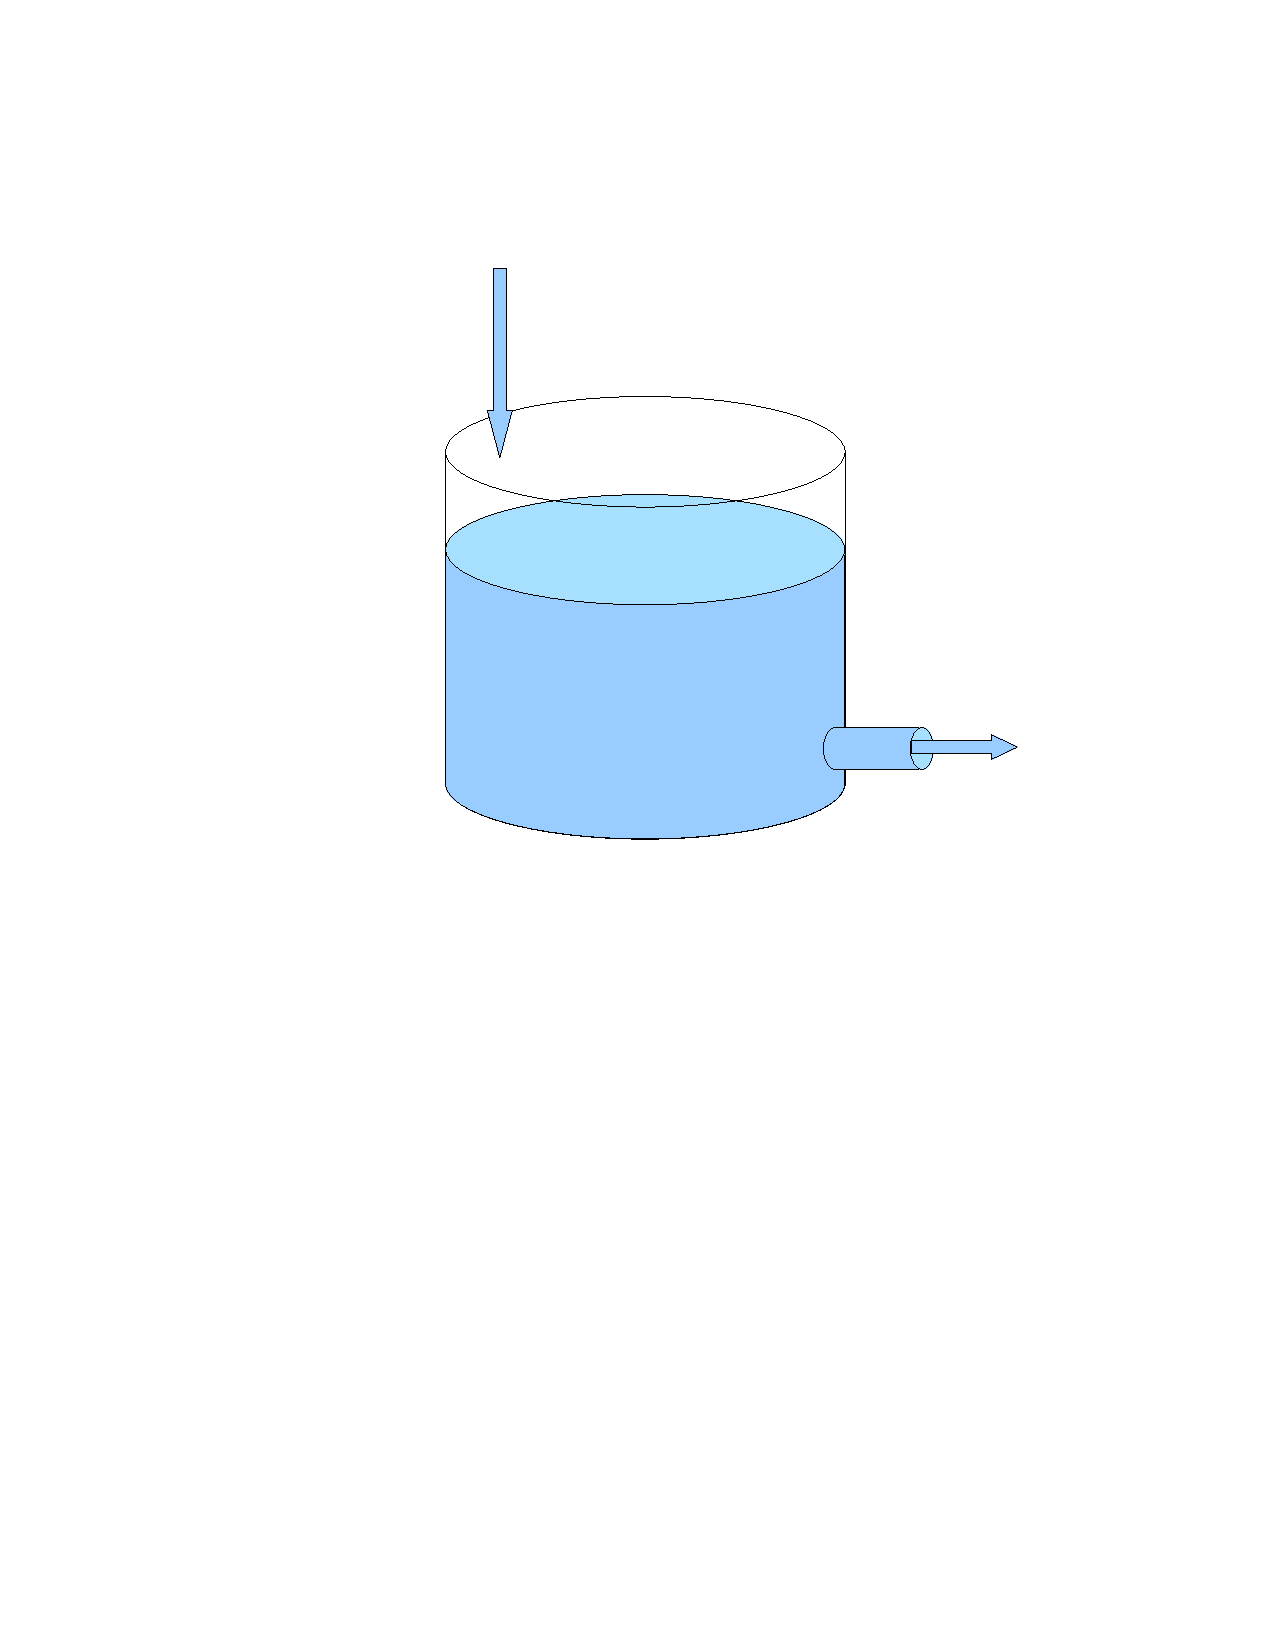
\includegraphics[width=0.45\textwidth]{fig1_midterm2007}
\caption{Situation modelled in exercise {\bf 1}.}
\label{fig:dilution}
\end{center}
\end{figure}
a tank contains initially, at time $t=0$, 100 litres of water. There is an inflow, at the rate of $r_{in}$ litres per minute, and an outflow at the rate of $r_{out}$ litres per minute. Before the experiment starts, the tank contains a concentration of salt of $C_0$. At the start of the experiment, liquid starts flowing into the tank, and the contents of the tank start flowing out.

\noindent
{\bf 1.a.}
Write a differential equation for the variation of the volume $V(t)$ of liquid in the tank at time $t$.

\noindent
{\bf 1.b.} 
Find the expression of $V(t)$, the volume of liquid in the tank at time $t$.

\noindent
{\bf 1.c.} Assume that $r_{in}=10$ litres per minute. What is the value of $r_{out}$, if after 1 hour, there remains exactly 50 litres of liquid in the tank.

\noindent
{\bf 1.d.} Assume now that $r_{in}=r_{out}$, so that the amount of liquid remains constant in the tank. Denote $r(t)$ this rate of in/out-flow, which we assume can vary with time. The inflow contains a concentration $S_0$ of salt. Assuming that the tank is well stirred, so that the concentration of salt is uniform in the tank, write a differential equation for the concentration $C(t)$ of salt in the tank at time $t$.

\noindent
{\bf 1.e.}
The general solution to the linear equation $x'+p(t)x=q(t)$ is given by 
\[
x(t)=e^{-\int p(t)dt}\left(\int e^{\int p(t)dt}q(t)dt+K\right),\quad K\in\mathbb{R}.
\]
Using this, solve the differential equation you found in {\bf 1.d}, with the initial condition $C(0)=C_0$.

\vskip1cm
\noindent
{\bf 2.} Consider the difference equation
\begin{equation}\label{eq:1}
x_{t+1}=\frac{ax_t}{b+x_t},
\end{equation}
with $a,b>0$ and $x_0\geq 0$.

\noindent{\bf 2.a.} Show that for $x_0\geq 0$, $x_t\geq 0$ for all $t$.

\noindent{\bf 2.b.} Find the fixed points of \eqref{eq:1}. 

\noindent{\bf 2.c.} Study the relevance (nonnegativity) and stability of these fixed points, as a function of the (relative) values of $a$ and $b$.

\noindent{\bf 2.d.} Summarize your findings of {\bf 2.c} in a diagram having $a$ on the $x$-axis (assuming a fixed value of $b$), and the value of the fixed points on the $y$-axis, as shown in Figure~\ref{fig:2}. Indicate an attracting equilibrium by a thick line, a repelling one by a dashed line.
\begin{figure}[htbp]
\begin{center}
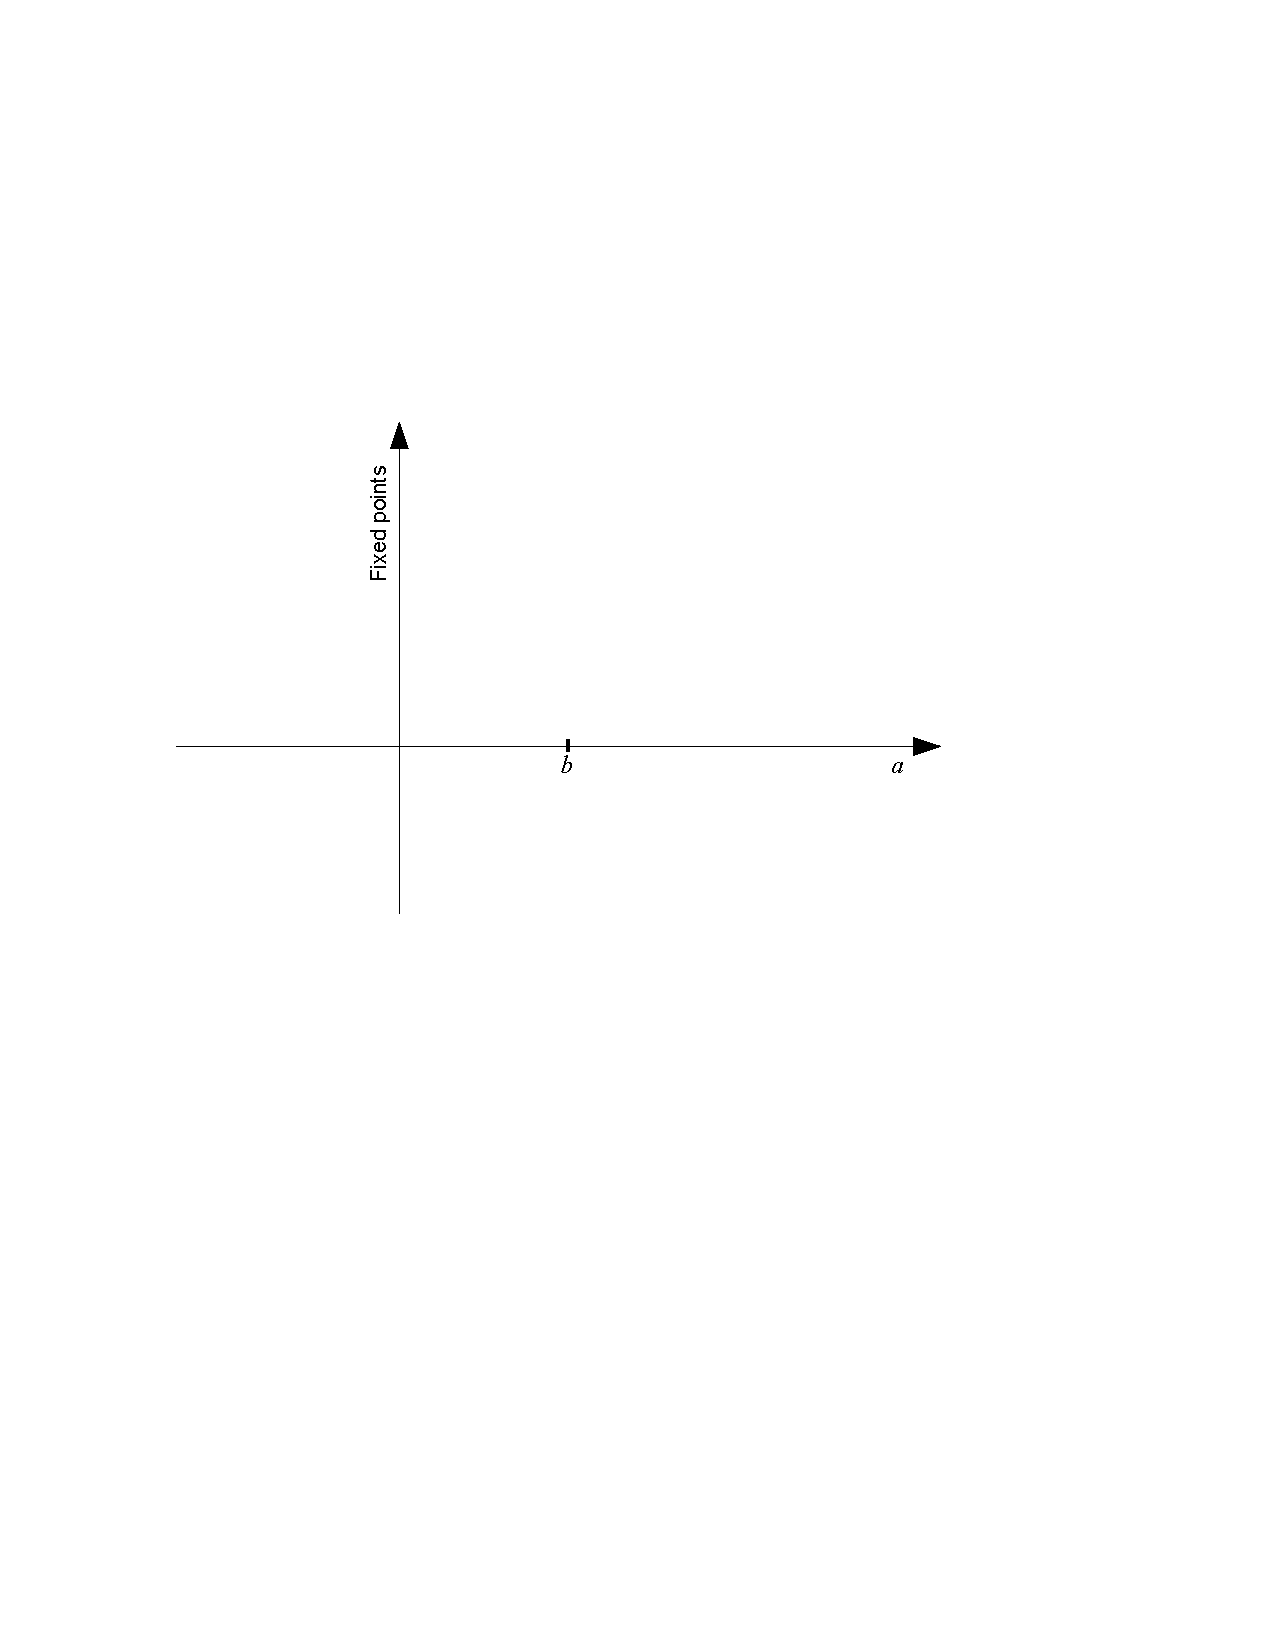
\includegraphics[width=0.45\textwidth]{fig2_midterm2007}
\caption{Setup of the bifurcation diagram for exercise {\bf 2.d}.}
\label{fig:2}
\end{center}
\end{figure}


\noindent{\bf 2.e.} Can \eqref{eq:1} have period 2 points other than its fixed points?


\vskip1cm
\noindent{\bf 3.}
Consider the following model for hares and fox, where $H(t)$ and $F(t)$ are the numbers of hares and fox at time $t$, respectively.
\begin{equation}\label{eq:2}
\begin{aligned}
H' &= (b_H-d_H)H - \pi HF \\
F' &= \sigma\pi HF -d_FF.
\end{aligned}
\end{equation}
The parameters are $b_H$, birth rate of hares, $d_H$, death rate of hares, $d_F$, death rate of fox, $\pi$, the predation rate, and $\sigma$, the conversion coefficient. We assume that $b_H,d_H,d_F>0$, while $\pi\geq 0$ and 
$0\leq\sigma\leq 1$. System \eqref{eq:2} is considered together with initial conditions $(H(0),F(0))=(H_0,F_0)$, with $H_0,F_0>0$.

\noindent{\bf 3.a.}
Suppose that there is no predation, i.e., $\pi=0$. Solve system \eqref{eq:2}, and discuss the behavior of its solutions as a function of the relative values of $b_H$ and $d_H$.

\noindent{\bf 3.b.}
Suppose now that $\pi>0$ and $\sigma>0$. Draw the nullclines of \eqref{eq:2}; show the direction field in each region of $\mathbb{R}_+^2$ hence delimited; identify the equilibria.

\noindent{\bf 3.c.}
Discuss the relevance (nonnegativity) and local stability of the equilibria, as a function of the relative values of $b_H$, $d_H$ and $d_F$, in the $\pi,\sigma>0$ case.


\end{document}